
\section{Experiments} \label{sec:exp}

{\SFOLowerUnits} has been implemented as a prototype\footnote{Source code available at \url{https://github.com/jgorzny/Skeptik}} in the functional programming language Scala\footnote{\url{http://www.scala-lang.org/}} as part of the \skeptik
 library\footnote{\url{https://github.com/Paradoxika/Skeptik}}. 
%{\LowerUnits} has been implemented as a recursive \FuncSty{delete} improvement.

The algorithm has been applied to 308 proofs produced by the {\SPASS}\footnote{\url{http://www.spass-prover.org/}} theorem prover on unsatisfiable benchmarks from the TPTP Problem Library\footnote{\url{http://www.cs.miami.edu/~tptp/}}. The proofs used were restricted to those which could be solved within 300 seconds by {\SPASS} on the Euler Cluster at the University of Victoria\footnote{\url{https://rcf.uvic.ca/euler.php}} using only the contraction and unifying resolution inference rules. The experiments were executed on a laptop (2.8GHz Intel Core i7 processor with 4 GB of RAM (1333MHz DDR3) available to the Java Virtual Machine), and the prototype implementation performed well on this system.



%For each proof $\psi$ (with the result of {\LowerUnits} applied to the proof denoted by $\alpha(\psi)$), the time to compress the proof ($t(\psi)$), the compression ratio ($(|\psi|-|\alpha(\psi)|)/|\psi|$), the resolution compression ratio  ($(|\psi|_R-|\alpha(\psi)|_R)/|\psi|_R$), the compression speed ($(|\psi|-|\alpha(\psi)|)/t(\psi)$), and resolution compression speed ($(|\psi|_R-|\alpha(\psi)|_R)/t(\psi)$) were measured\footnote{The raw data is available at \url{https://docs.google.com/spreadsheets/d/1F1-t2OuhypmTQhLU6yTj42aiZ5CqqaZvhVvOzeFgn0k/edit\#gid=1182923972}}, where $|\psi|_R$ indicates the number of resolution inference rules in the proof $\psi$.

%we don't have time charts. we can stop talking about that?
For each proof $\psi$ (with the result of {\SFOLowerUnits} applied to the proof denoted by $\alpha(\psi)$), the time to compress the proof ($t(\psi)$) and the resolution compression ratio  ($(|\psi|_R-|\alpha(\psi)|_R)/|\psi|_R$) were measured\footnote{The raw data is available at \url{https://docs.google.com/spreadsheets/d/1F1-t2OuhypmTQhLU6yTj42aiZ5CqqaZvhVvOzeFgn0k/edit\#gid=1182923972}}, where $|\psi|_R$ indicates the number of resolution inference rules in the proof $\psi$.

%Figure \ref{} shows the compression time $t(\psi)$ for each proof, sorted by proof length, and figure \ref{} (respectively figure \ref{}) shows the compression speed (respectively resolution compression speed) for each proof, also sorted by proof length

Figure \ref{fig:ex} (a) shows the average compression ratio sorted by proof length without the uncompressed proofs, and the average including the uncompressed proofs (b). Uncompressed proofs are those which had no valid units to lower or for which \SFOLowerUnits returned the original proof (there were 14 such proofs). In the longer proofs, there appear to be more valid units to lower, and these could reduce the number of resolutions in the proof by as much as 20\%.

Figure \ref{fig:ex} (c) shows the number of proofs of each length compressed and the combined number of proof nodes before and after compression (e). Note that there is a trend that as the length of the proof increases, a higher percentage of proofs can be compressed. This is expected, as larger proofs are more likely to include more valid unit clauses. The total number of proof nodes starts to drop of quickly once these larger proofs are accounted for. Figure \ref{fig:ex} (f) provides a better look at this behavior on the left; as a result of about the last 20 proofs, over 500 proof nodes are saved. Figure \ref{fig:ex} (d) shows the original proof length compared against the compressed proof length on the right.


% \begin{figure}
% 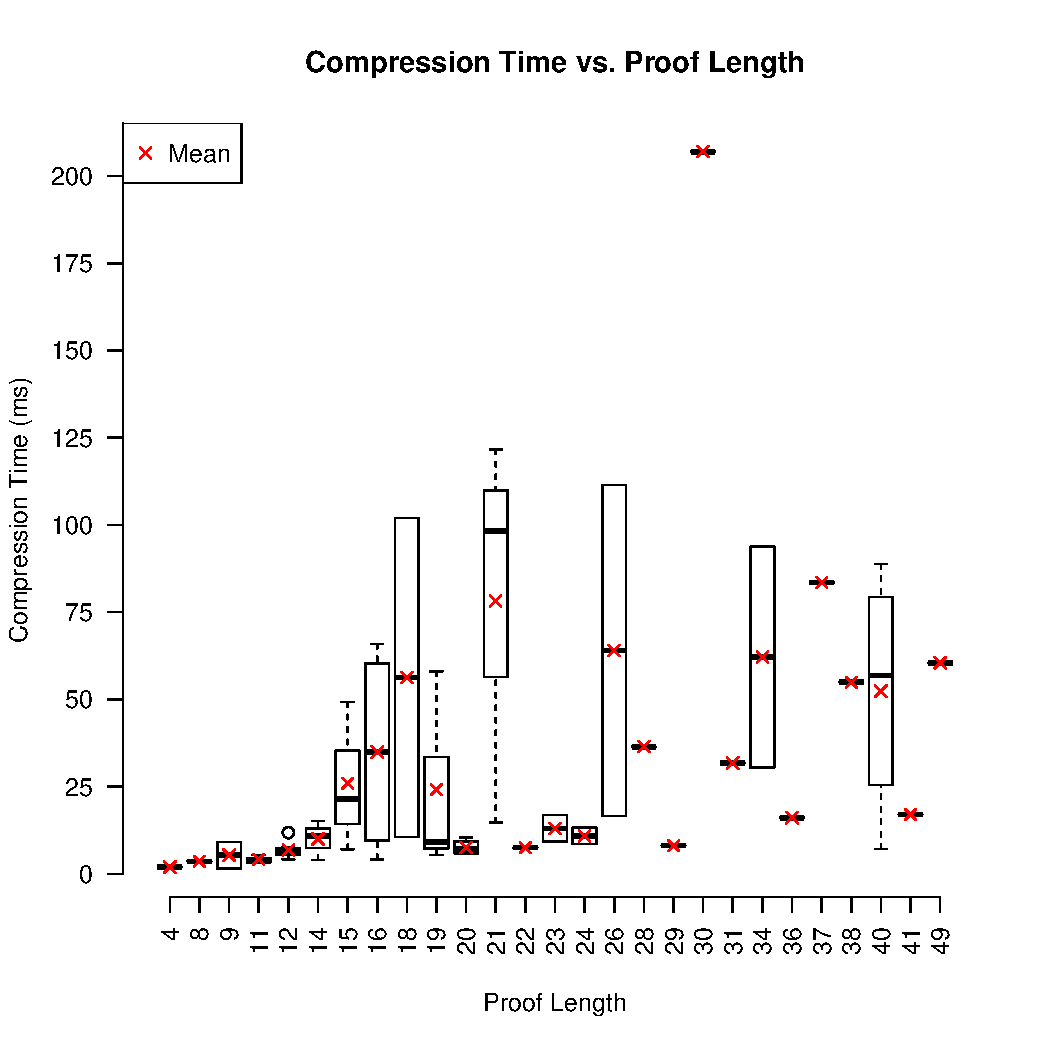
\includegraphics[scale=0.5]{images/compress_time_vs_proof_length.pdf}
% \end{figure}

% \begin{figure}
% 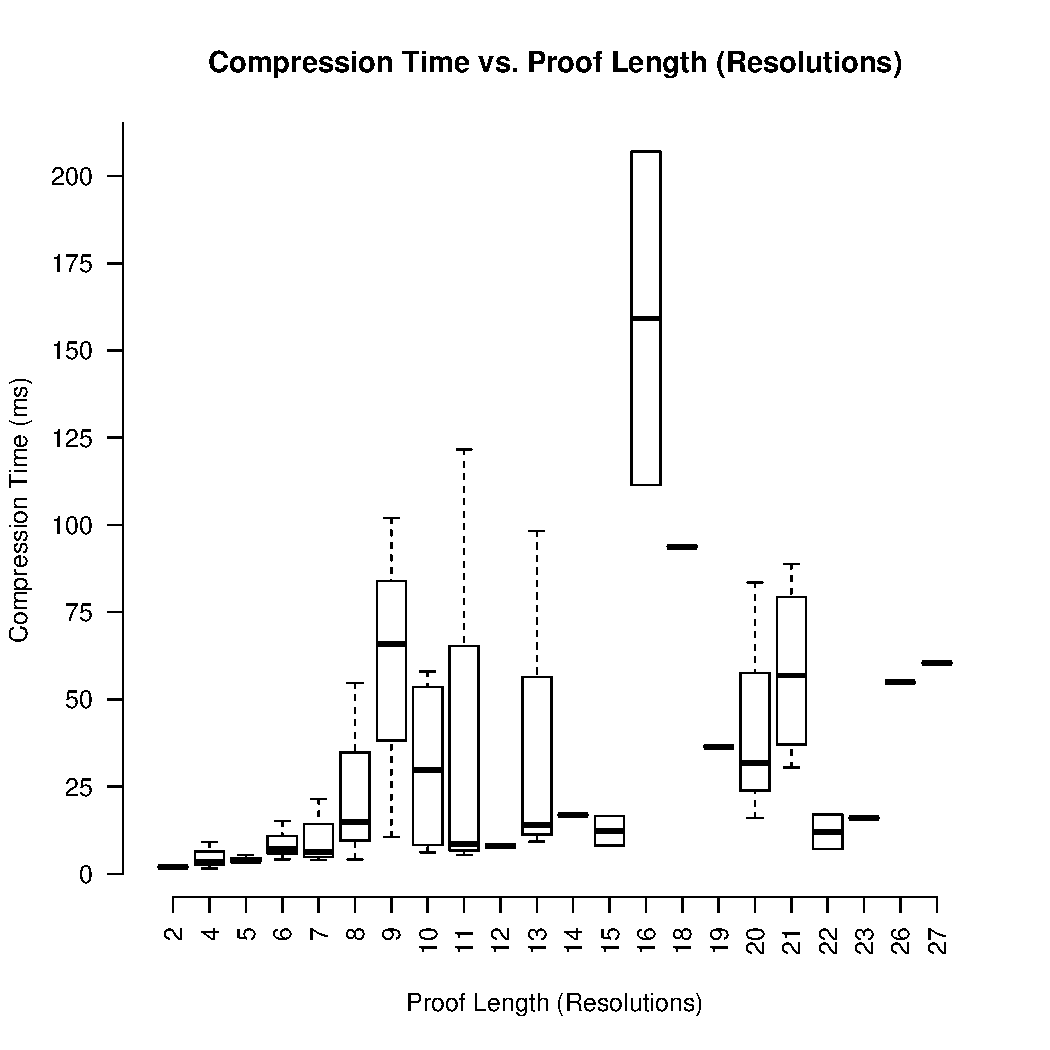
\includegraphics[scale=0.5]{images/compress_time_vs_proof_length_res.pdf}
% \end{figure}

% \begin{figure}
% 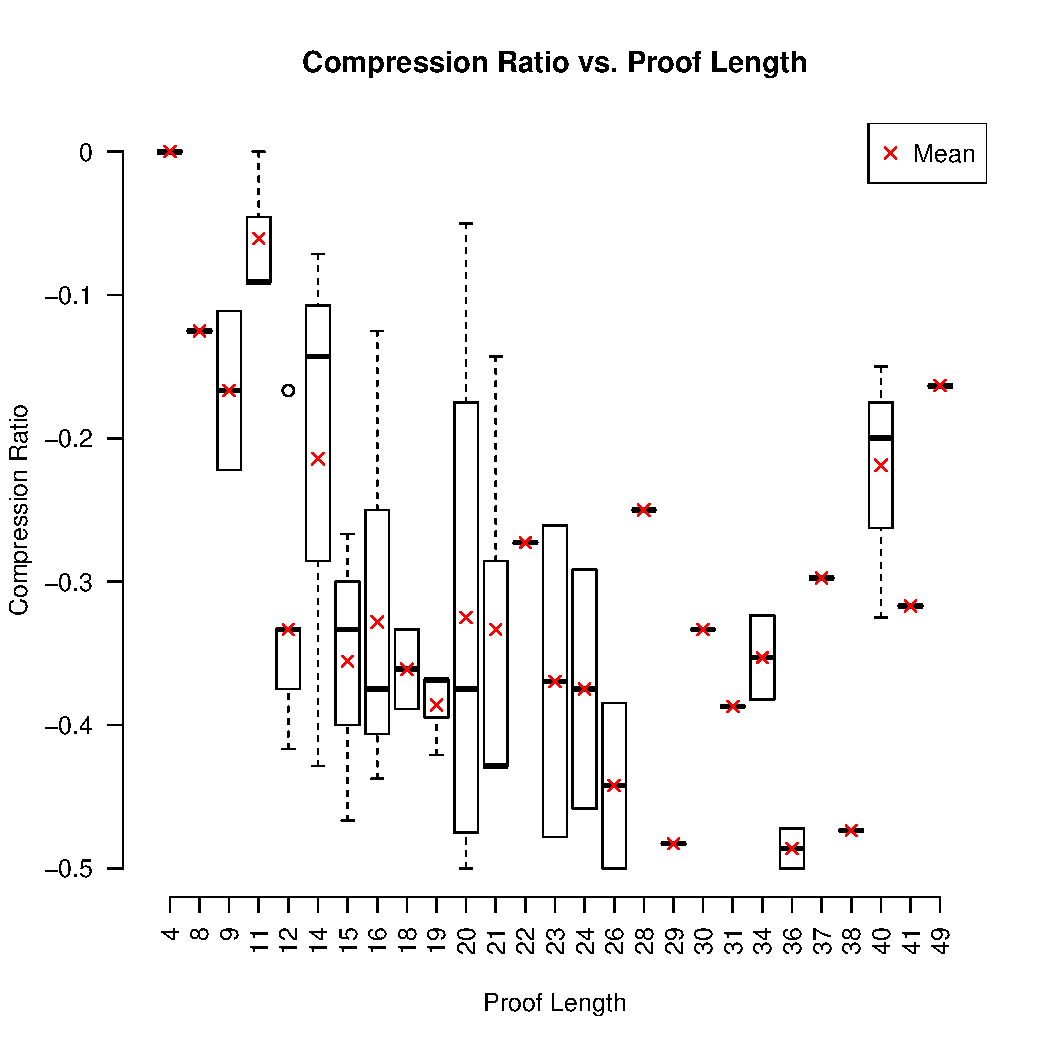
\includegraphics[scale=0.5]{images/compress_ratio_vs_proof_length.pdf}
% \end{figure}

%\begin{figure}\label{fig:compressRatioResVLength} %USED
%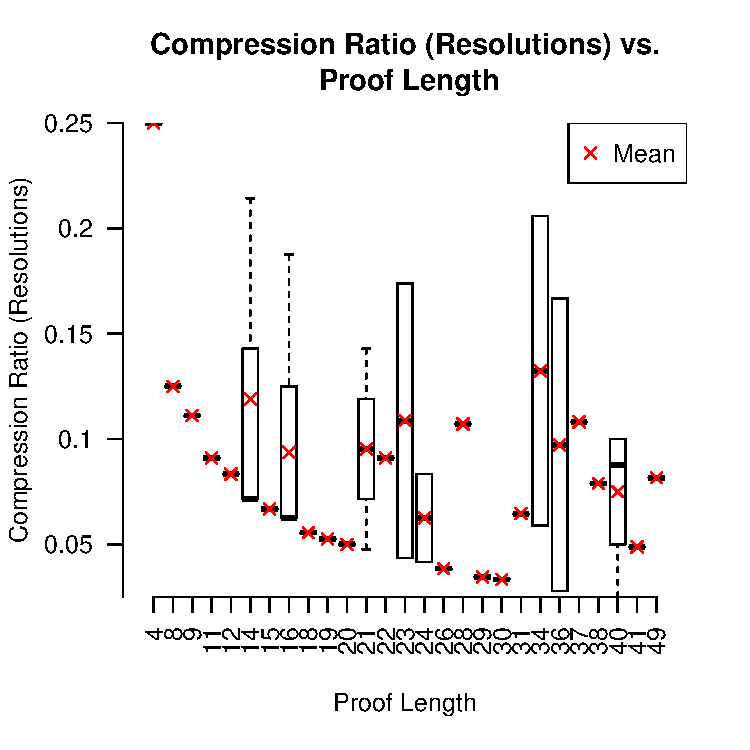
\includegraphics[scale=0.5]{images/compress_ratio_res_vs_proof_length.pdf}
%\end{figure}

% \begin{figure}
% 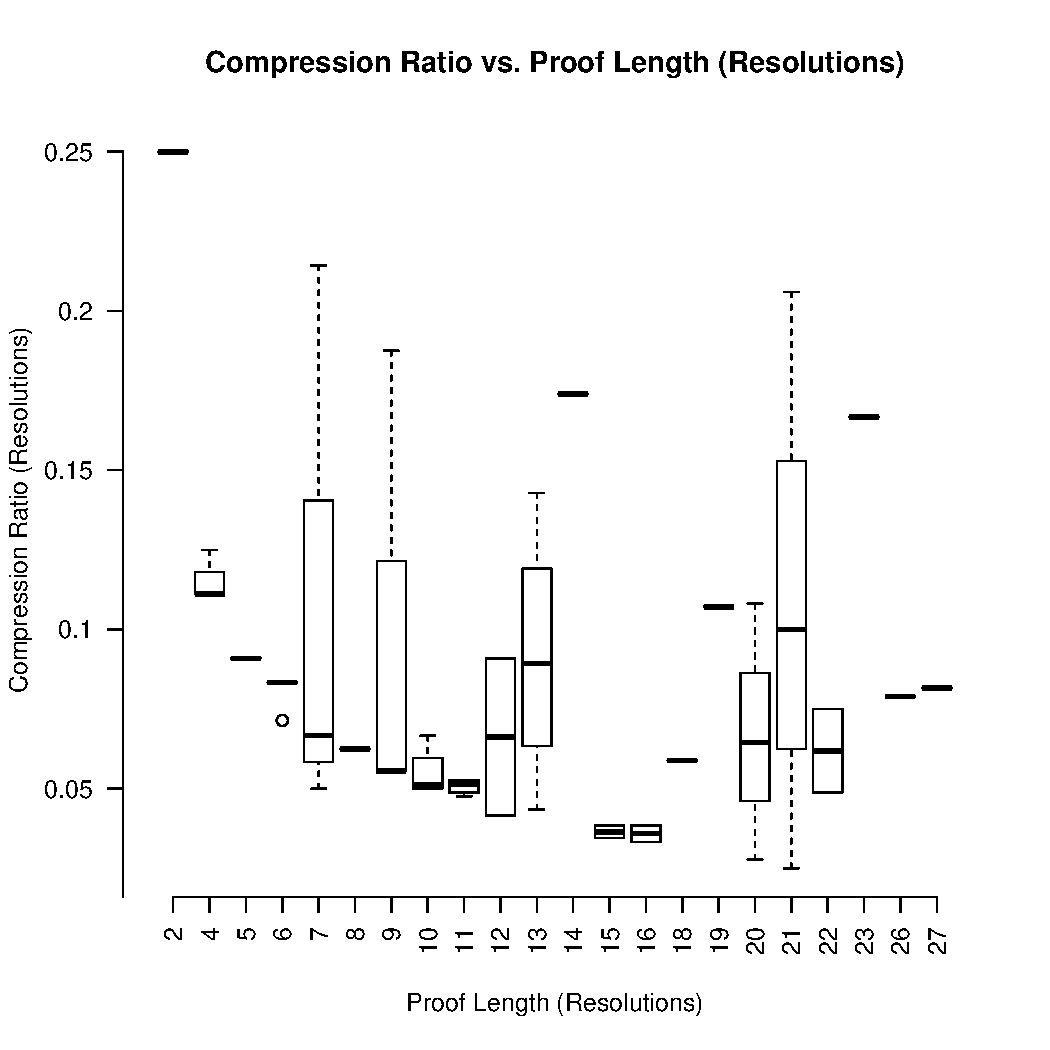
\includegraphics[scale=0.5]{images/compress_ratio_res_vs_proof_length_res.pdf}
% \end{figure}

%\begin{figure}%USED
%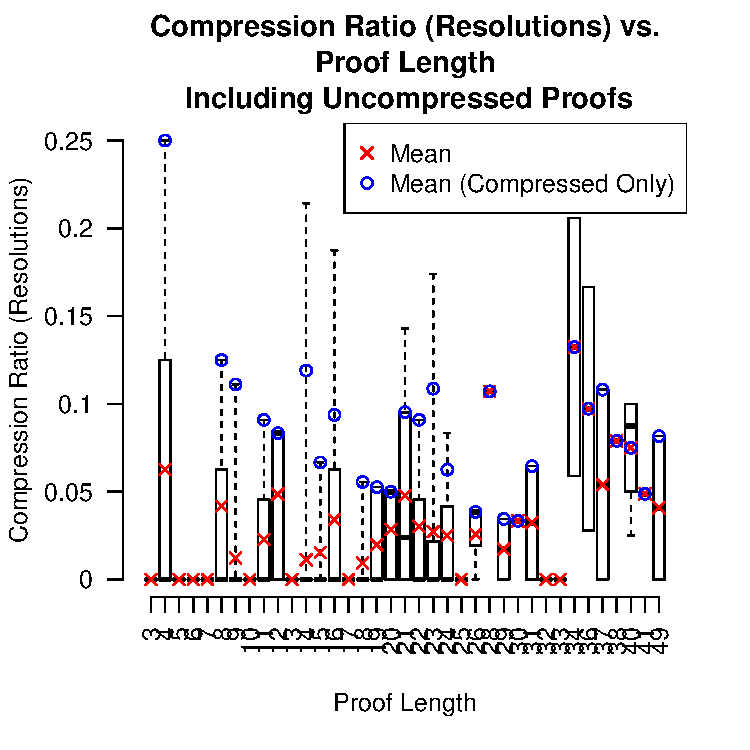
\includegraphics[scale=0.5]{images/compress_ratio_res_vs_proof_length_all_proofs.pdf}
%\end{figure}
\begin{figure}
\centering
%    \subfloat[Average compression (only success)]{{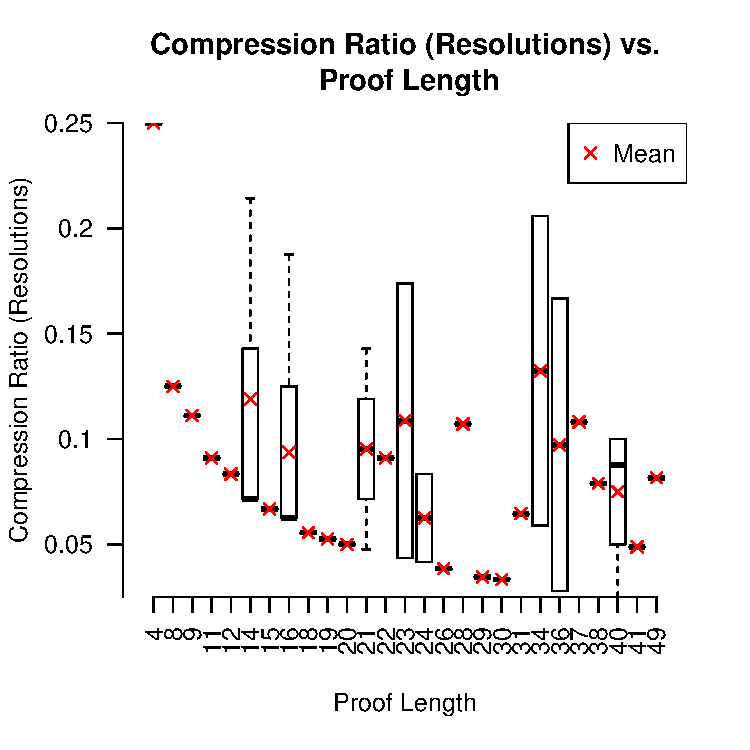
\includegraphics[scale=0.5]{images/compress_ratio_res_vs_proof_length.pdf} }}
    \subfloat[Overall average compression]{{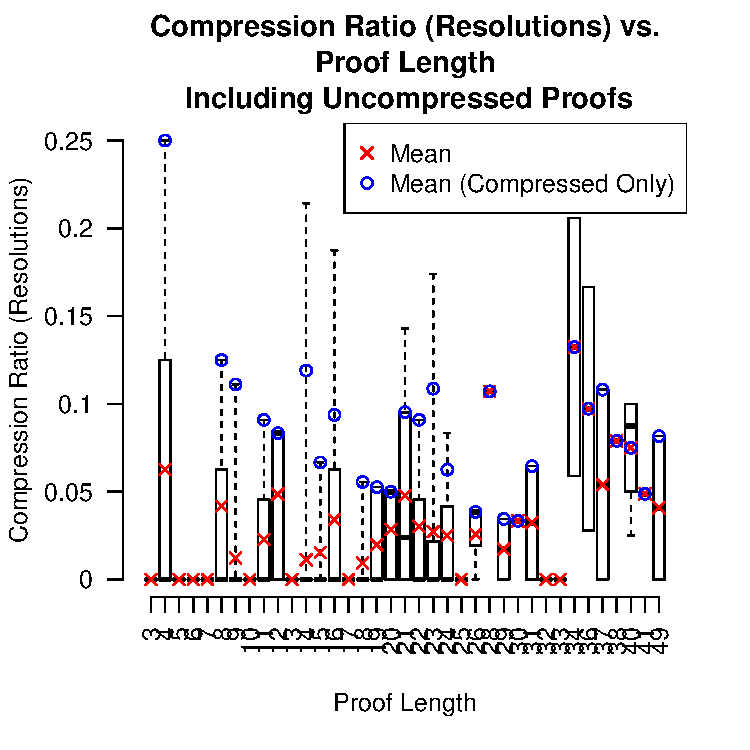
\includegraphics[scale=0.5]{images/compress_ratio_res_vs_proof_length_all_proofs.pdf} }}%\hfilll
    \subfloat[Number of proofs of each length compressed]{{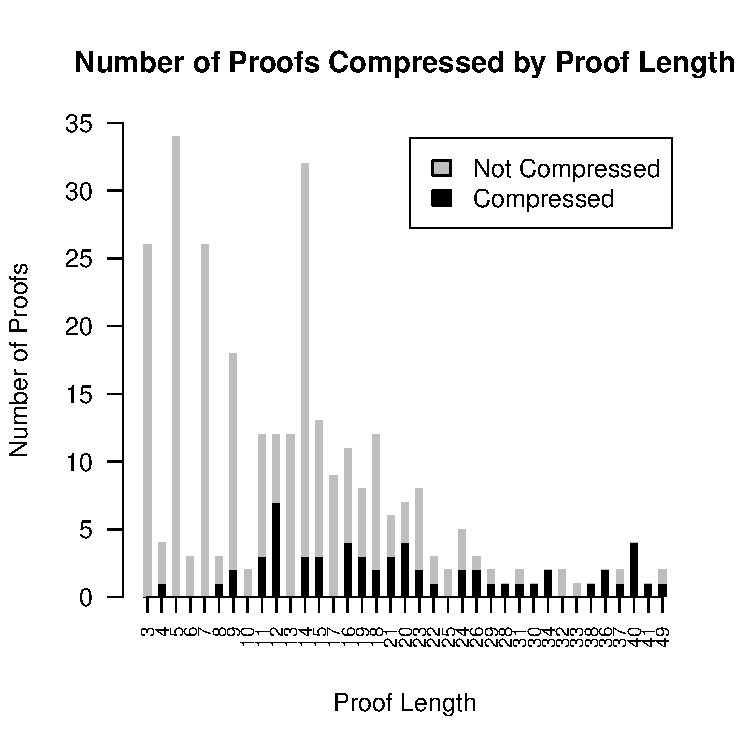
\includegraphics[scale=0.5]{images/num_compressed_stacked.pdf}}}\hfill
    \subfloat[Compressed length against input length]{{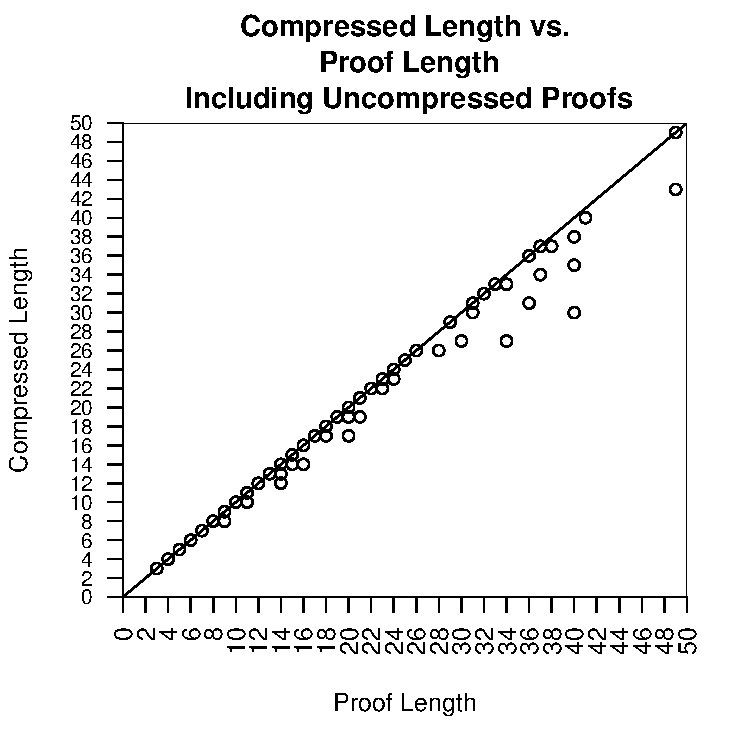
\includegraphics[scale=0.5]{images/compress_length_no_sub_vs_length_all_proofs.pdf} }}
%    \subfloat[Total proof nodes]{{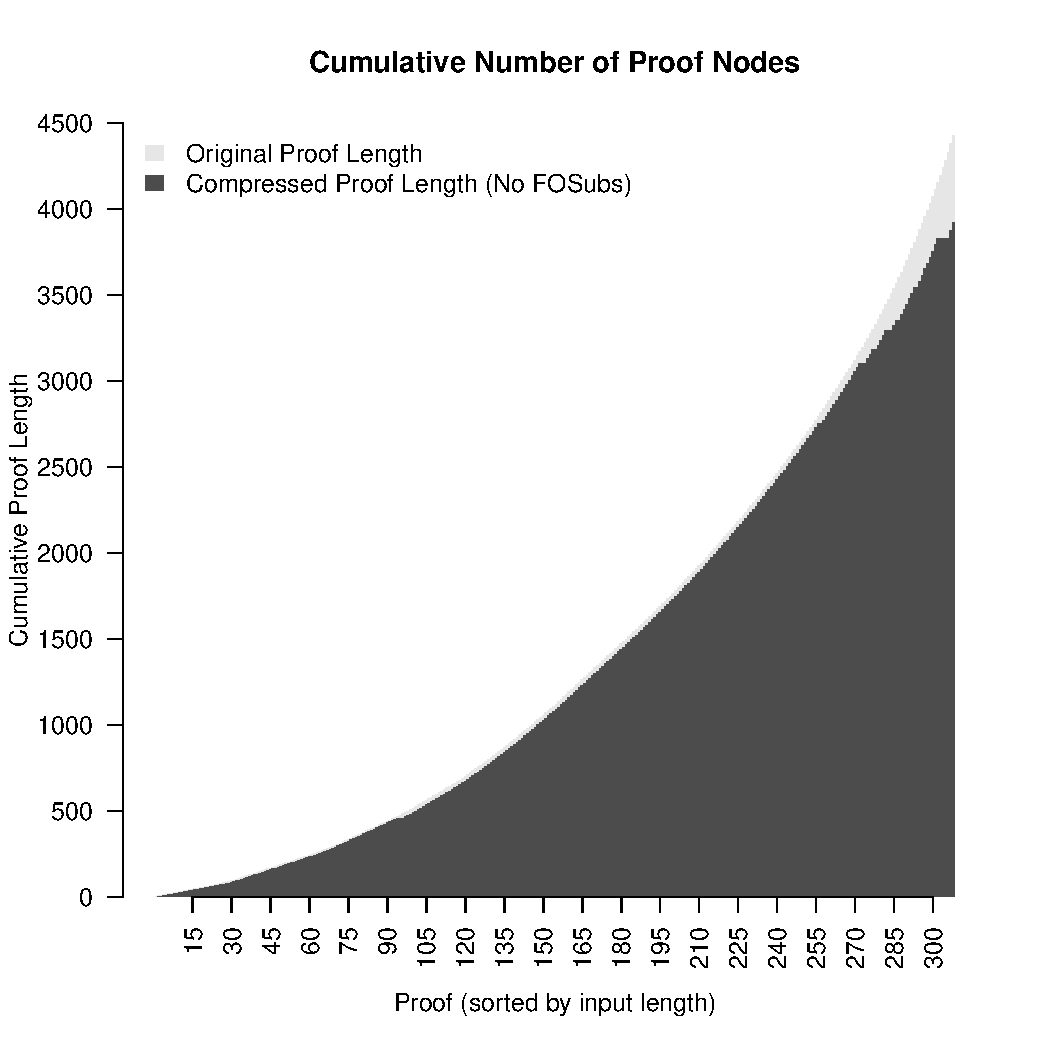
\includegraphics[scale=0.5]{images/cumulative_res_nodes_no_subs.pdf} }}
    \subfloat[Node reduction resulting from 100 largest proofs]{{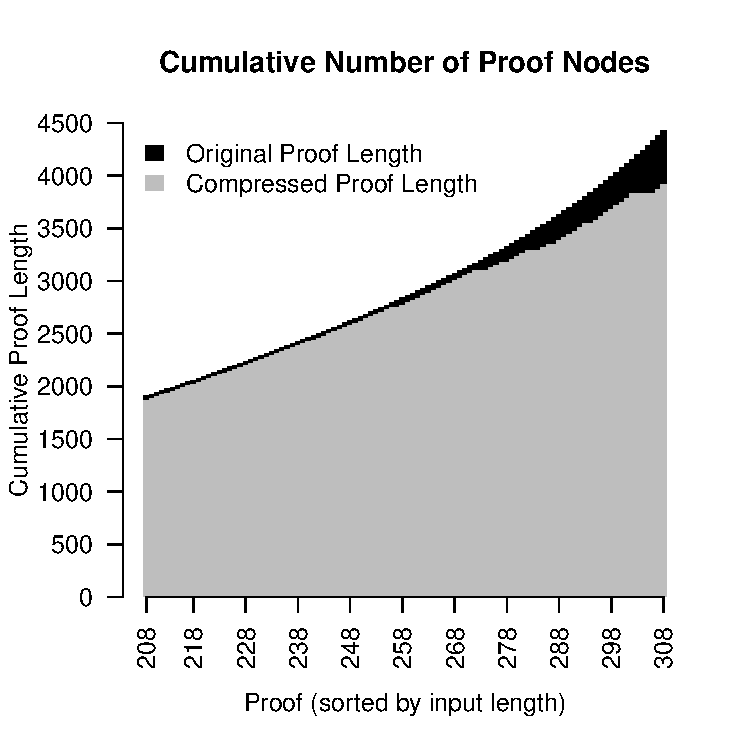
\includegraphics[scale=0.5]{images/cumulative_res_nodes_no_subs_top100.pdf}}}
\caption{Empirical evaluation results.}
\label{fig:ex}
\end{figure}


%\begin{figure}
%\centering
%    \subfloat{{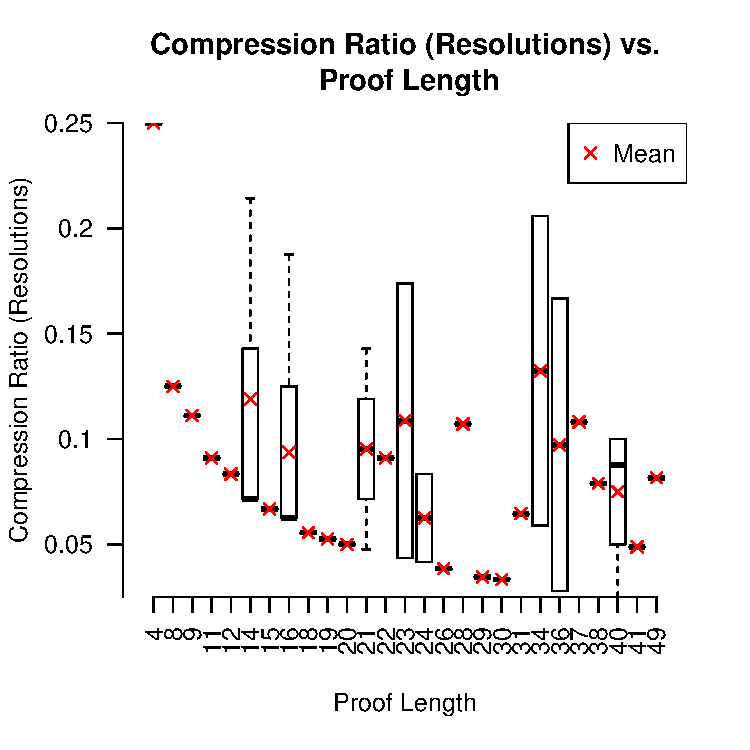
\includegraphics[scale=0.5]{images/compress_ratio_res_vs_proof_length.pdf}
%}}%
%    \subfloat{{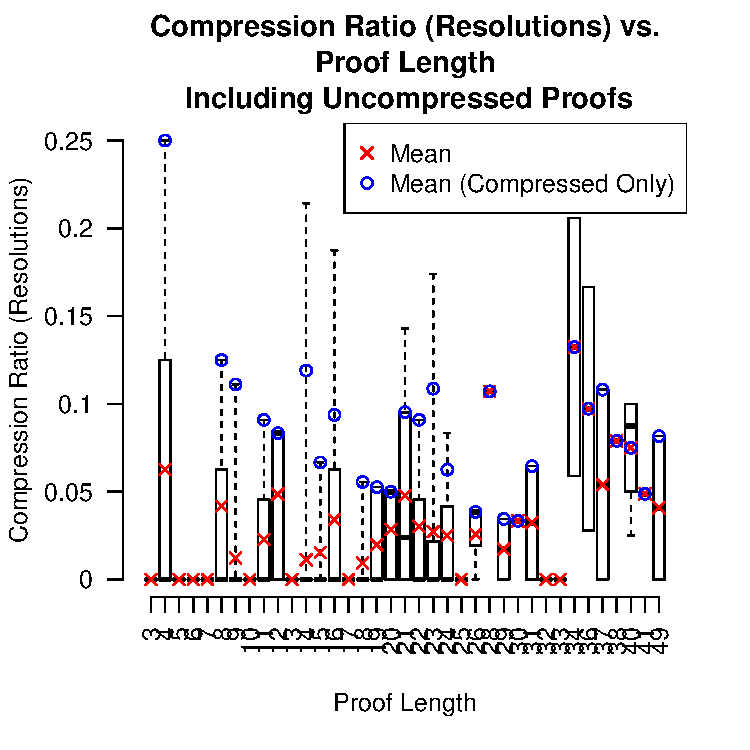
\includegraphics[scale=0.5]{images/compress_ratio_res_vs_proof_length_all_proofs.pdf} }}%
%\caption{Compression ratio versus proof length without uncompressed proofs (left) and with with uncompressed proofs (right).}
%\label{fig:ex1}
%\end{figure}



% \begin{figure}
% 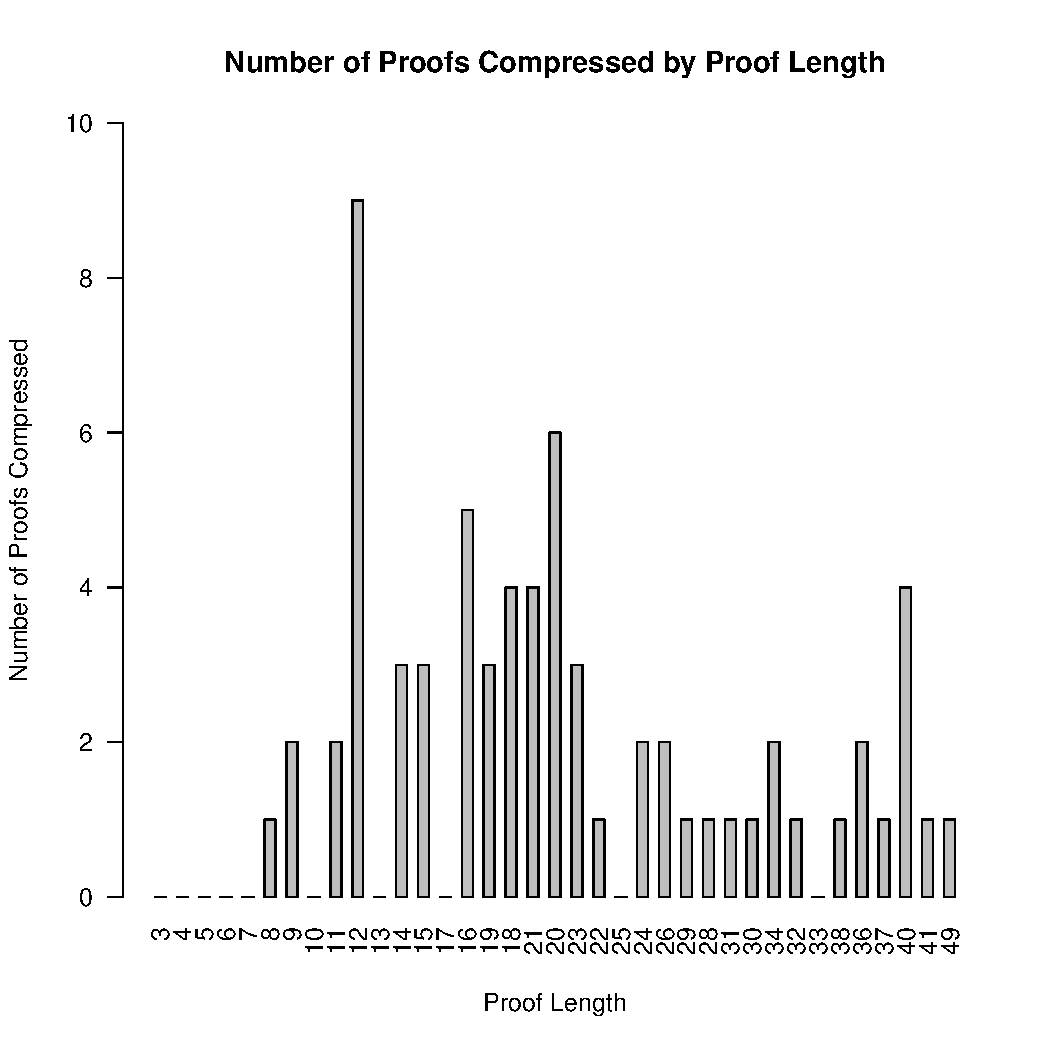
\includegraphics[scale=0.5]{images/num_compressed_count.pdf}
% \end{figure}

% \begin{figure}
% 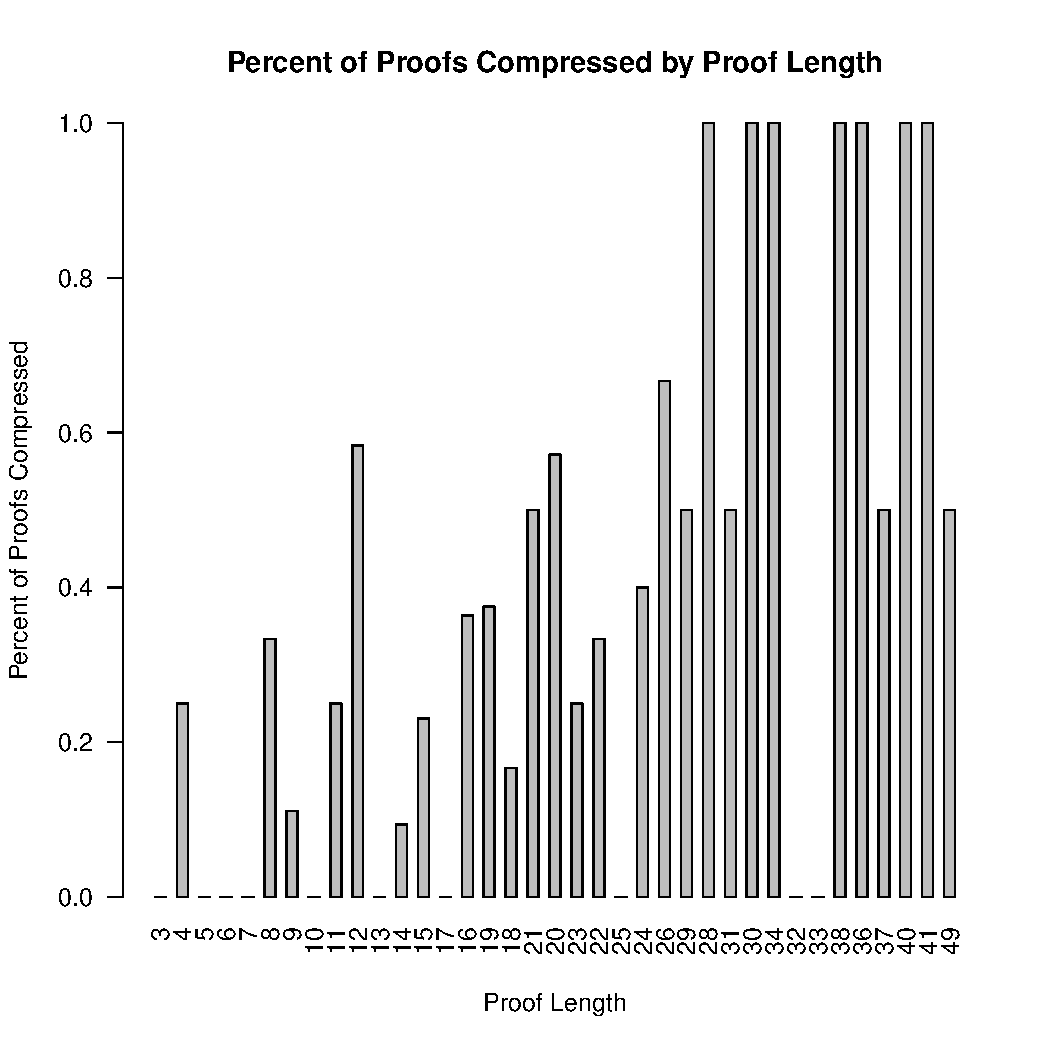
\includegraphics[scale=0.5]{images/num_compressed_percent.pdf}
% \end{figure}


%\begin{figure}%USED
%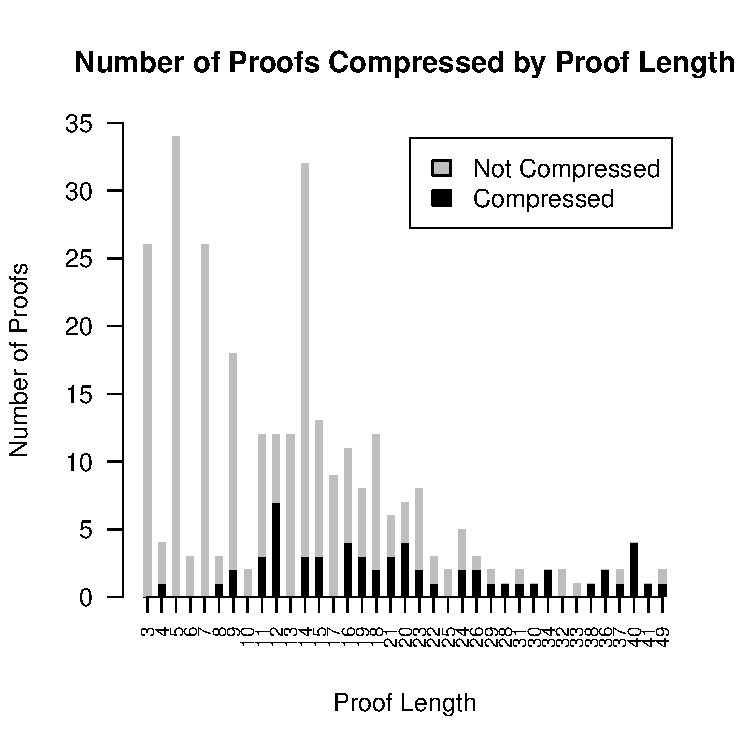
\includegraphics[scale=0.5]{images/num_compressed_stacked.pdf}
%\end{figure}

%\begin{figure}
%\centering
%    \subfloat{{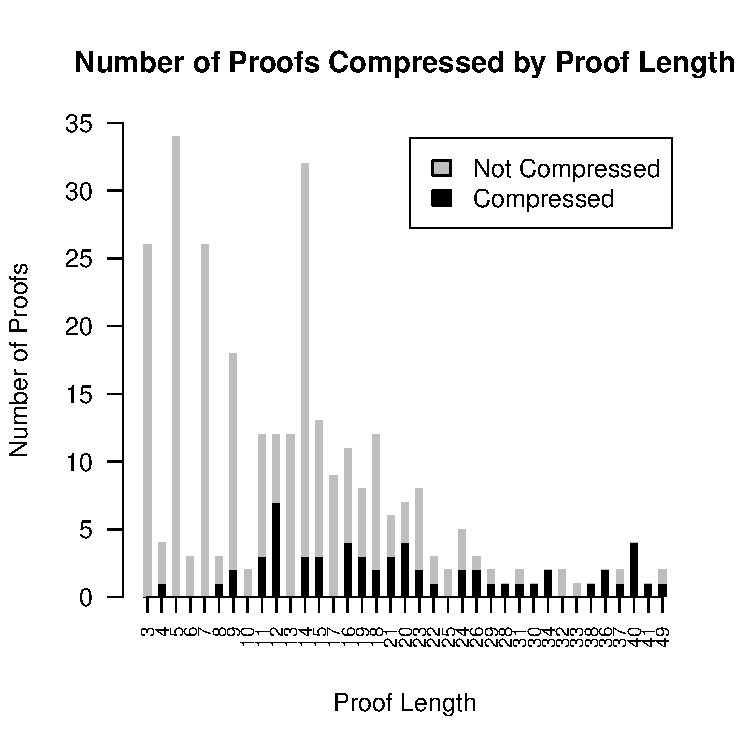
\includegraphics[scale=0.5]{images/num_compressed_stacked.pdf}
%}}%
%    \subfloat{{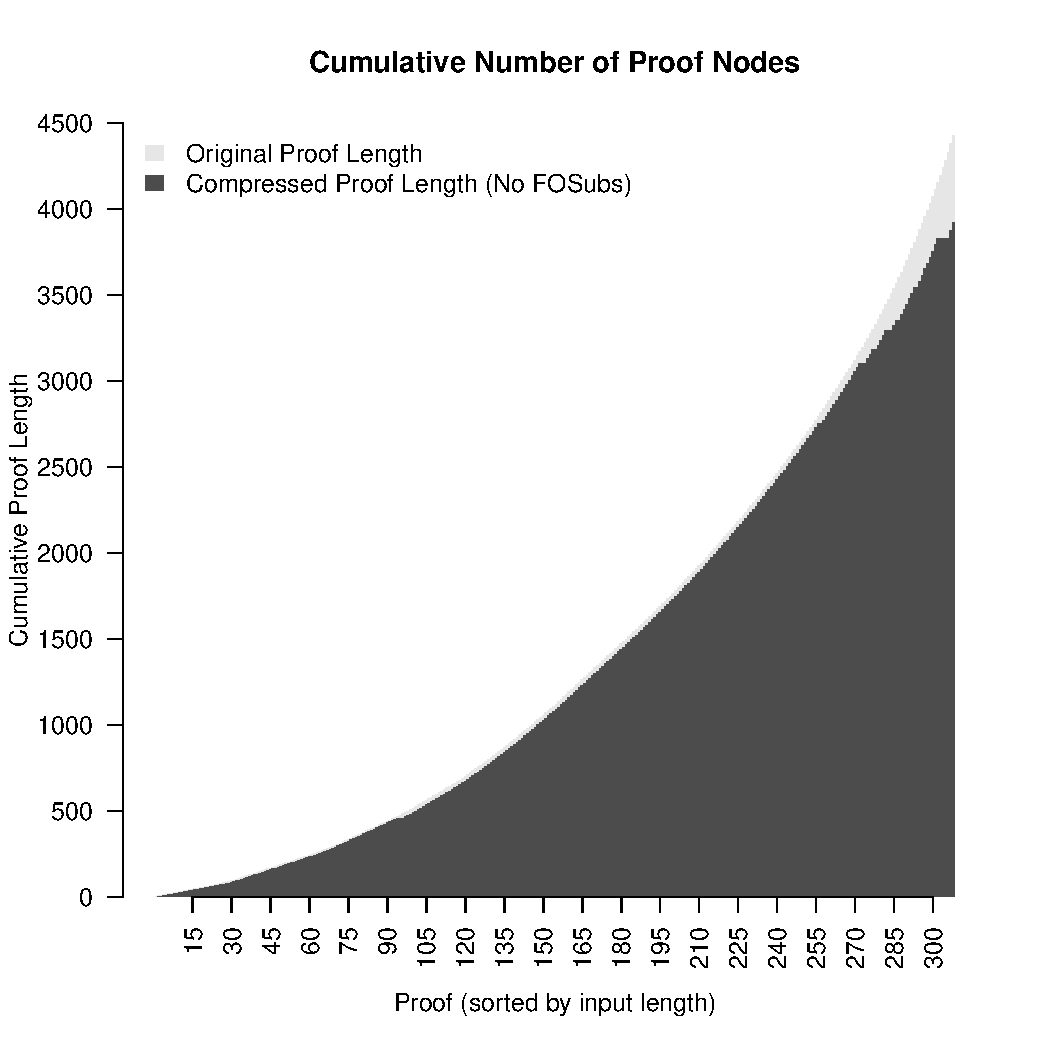
\includegraphics[scale=0.5]{images/cumulative_res_nodes_no_subs.pdf} }}
%\caption{Number of proofs compressed of each length (left), and total number of nodes before and after compression (right).}
%\label{fig:ex2}
%\end{figure}


% \begin{figure}
% 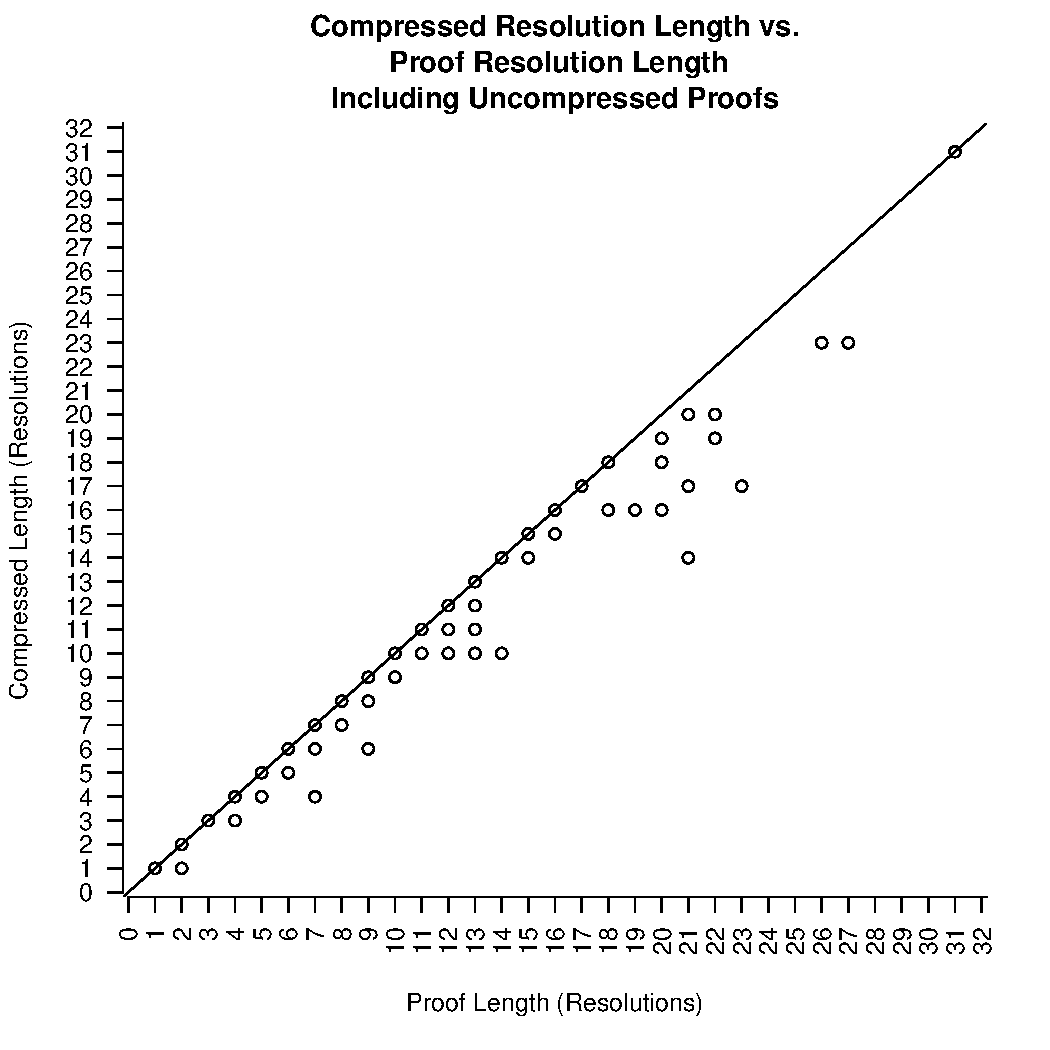
\includegraphics[scale=0.5]{images/res_length_vs_compress_res_length_all_proofs.pdf}
% \end{figure}
% \begin{figure}
% 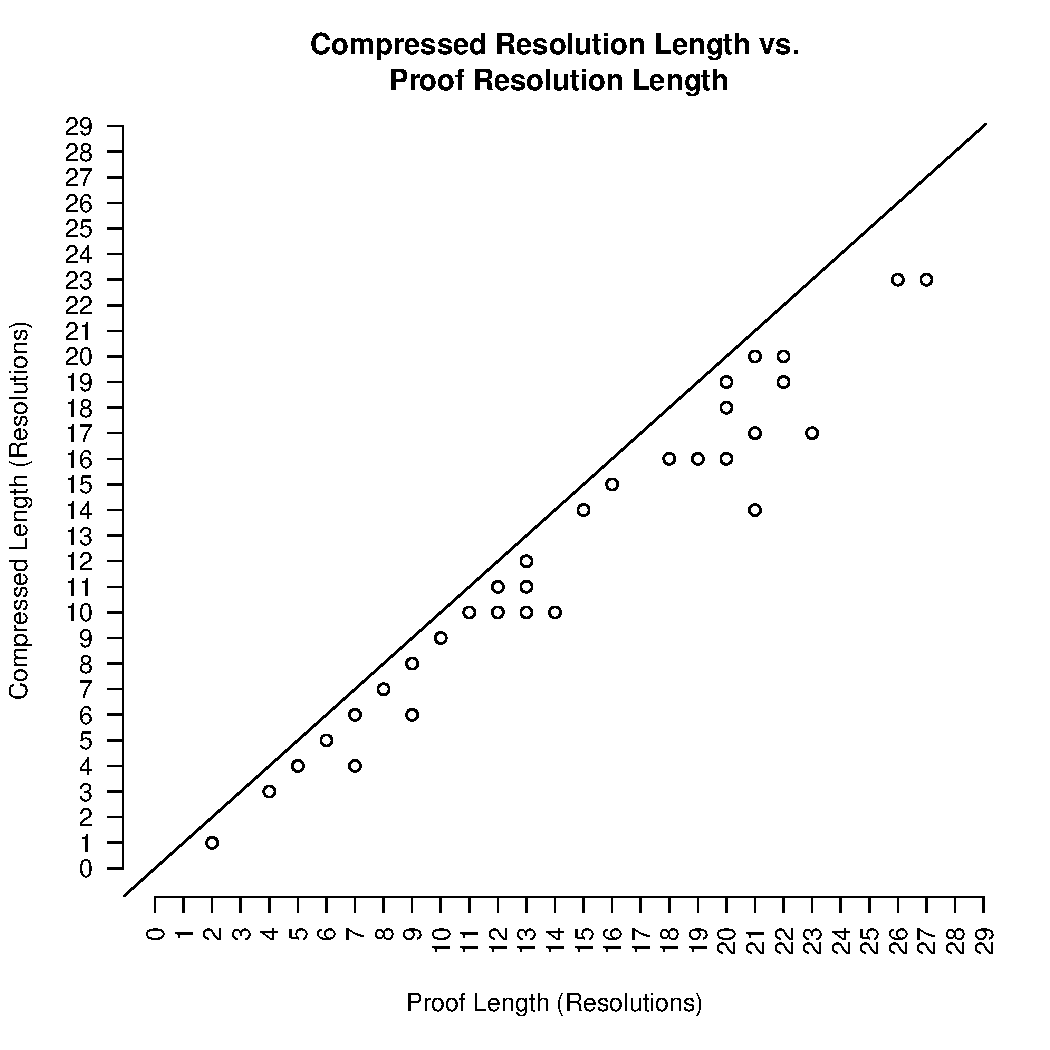
\includegraphics[scale=0.5]{images/res_length_vs_compress_res_length.pdf}
% \end{figure}

% \begin{figure}
% 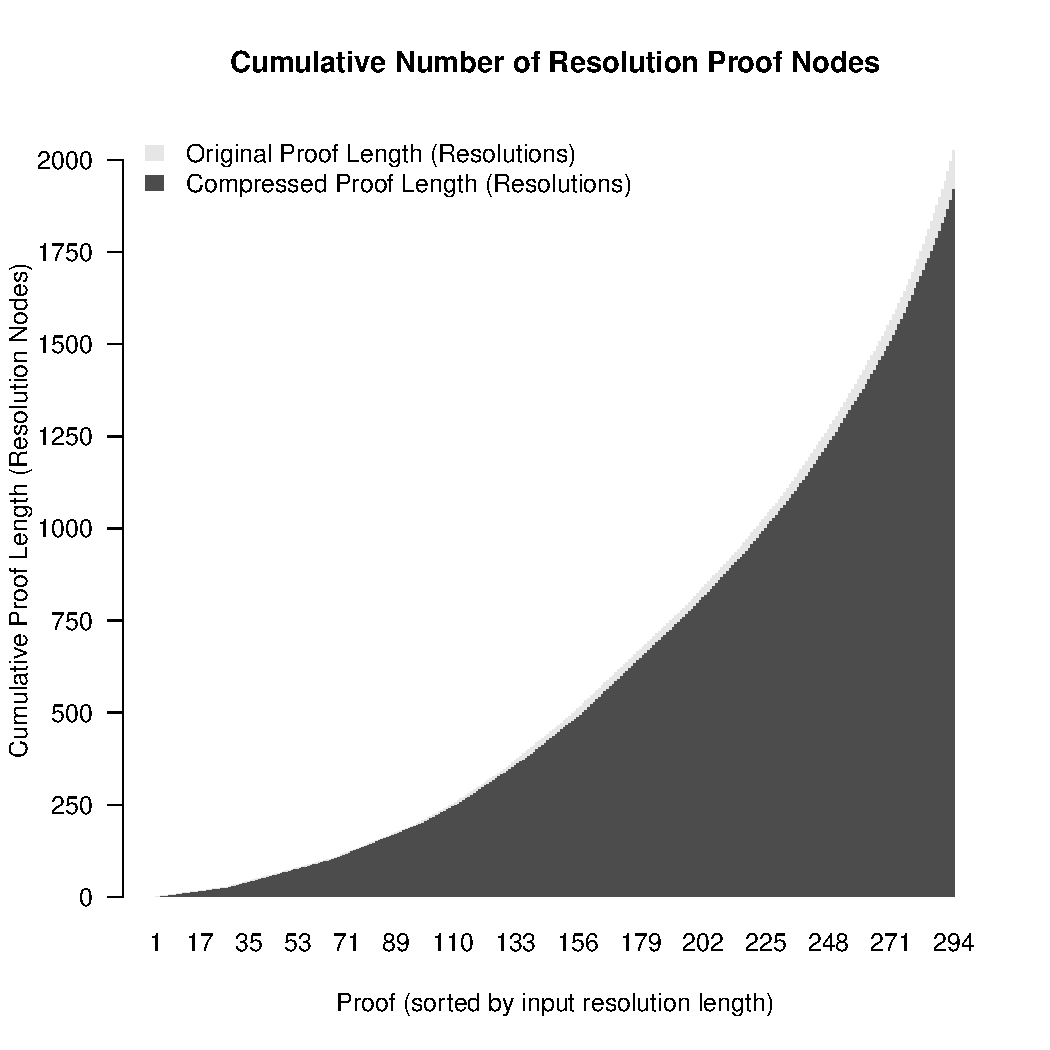
\includegraphics[scale=0.5]{images/cumulative_res_nodes.pdf}
% \end{figure}

%\begin{figure}%USED
%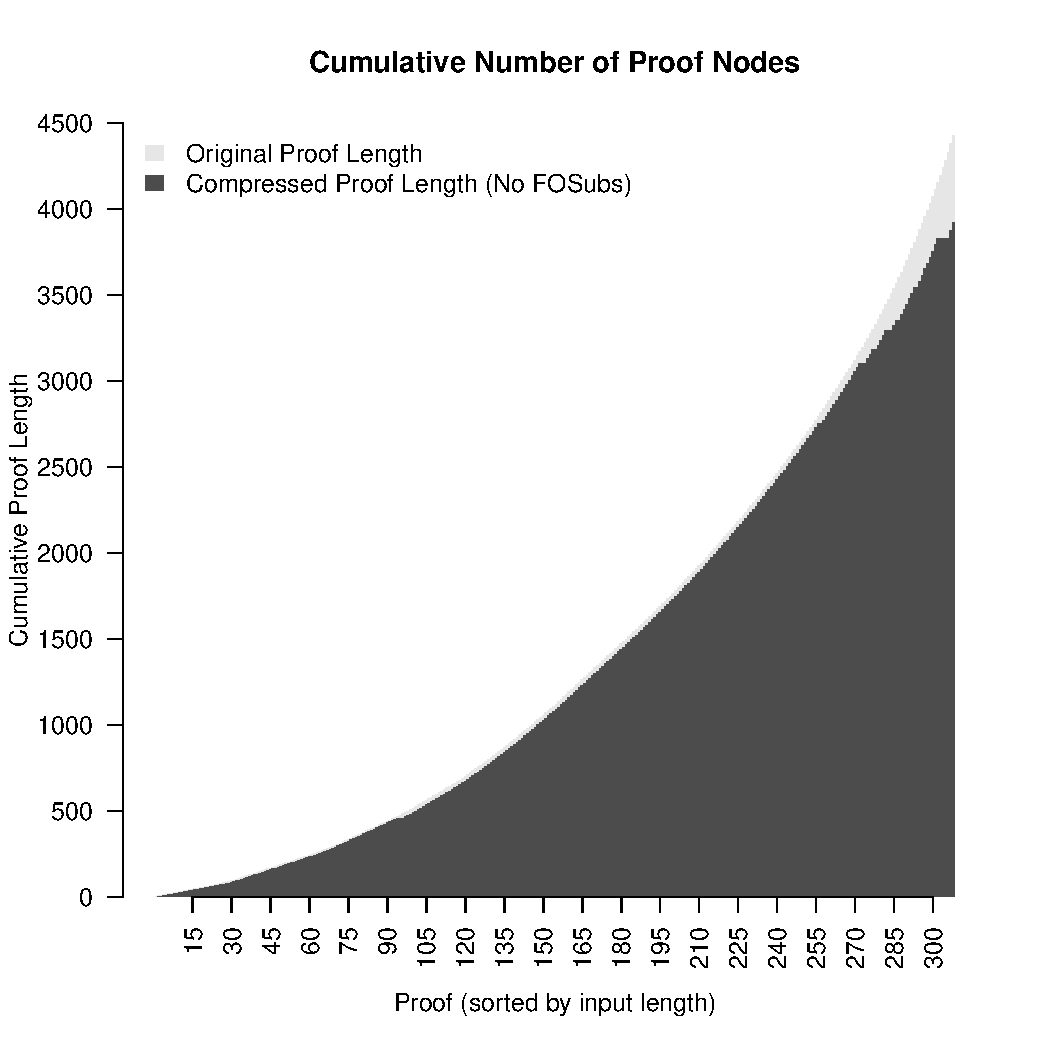
\includegraphics[scale=0.5]{images/cumulative_res_nodes_no_subs.pdf}
%\end{figure}

%\begin{figure} %USED
%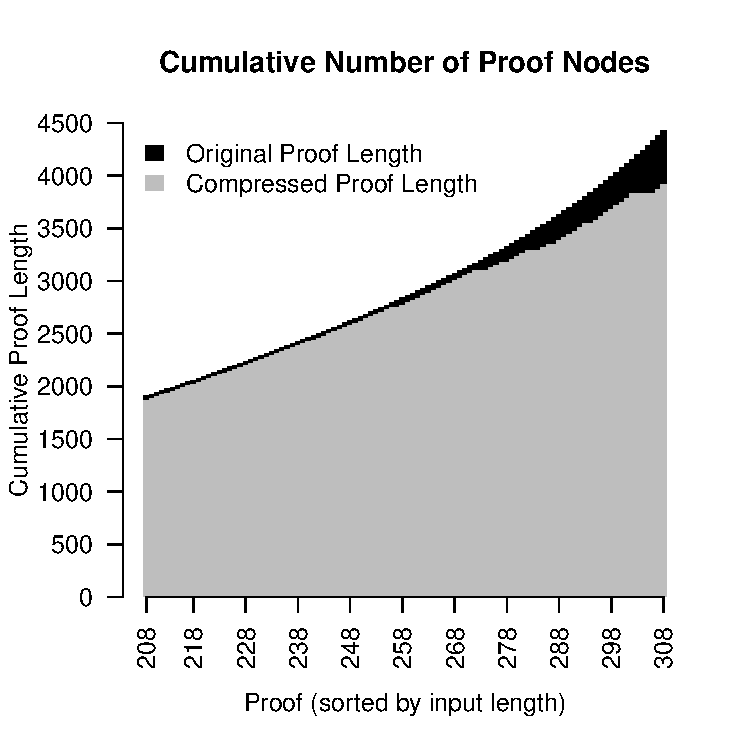
\includegraphics[scale=0.5]{images/cumulative_res_nodes_no_subs_top100.pdf}
%\end{figure}




% \begin{figure}
% 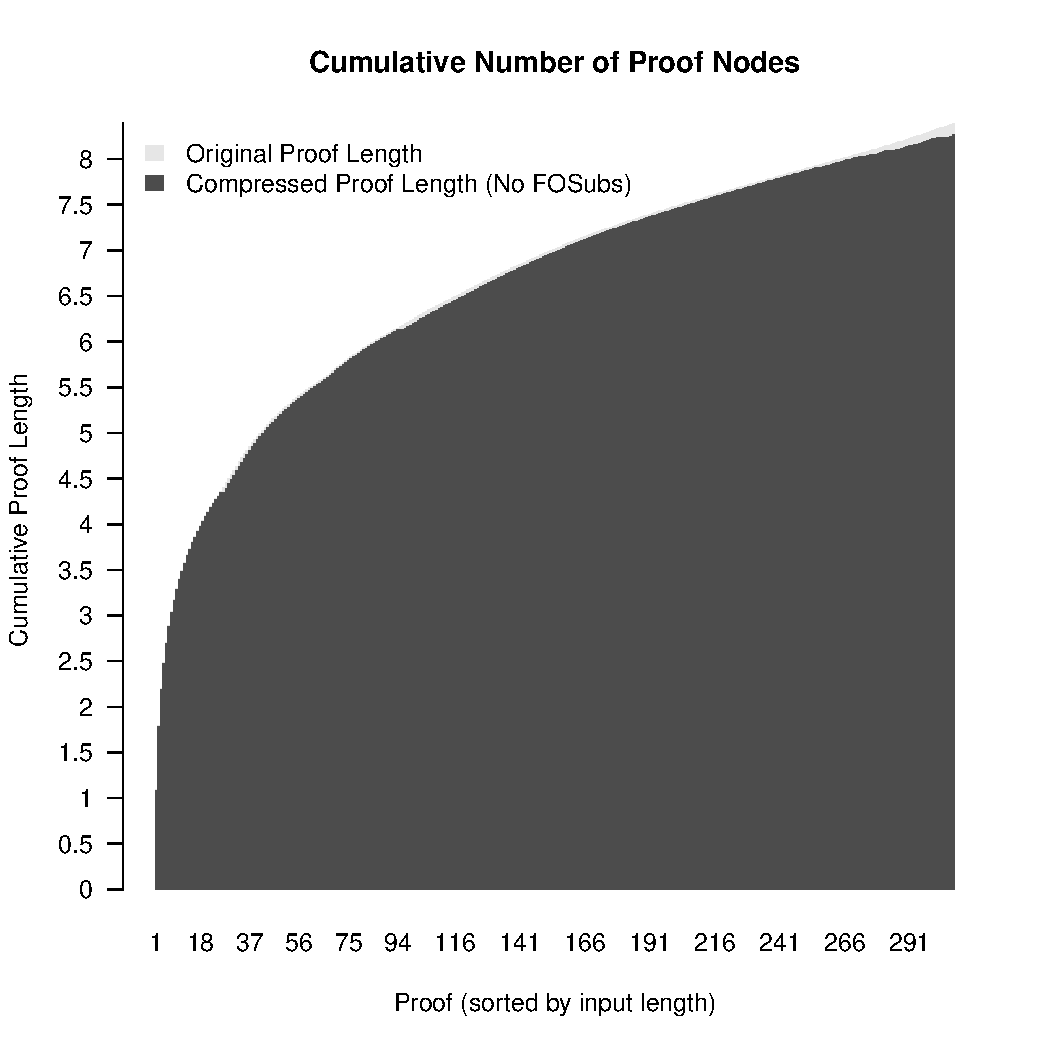
\includegraphics[scale=0.5]{images/cumulative_res_nodes_no_subs_log.pdf}
% \end{figure}
% \begin{figure}
% 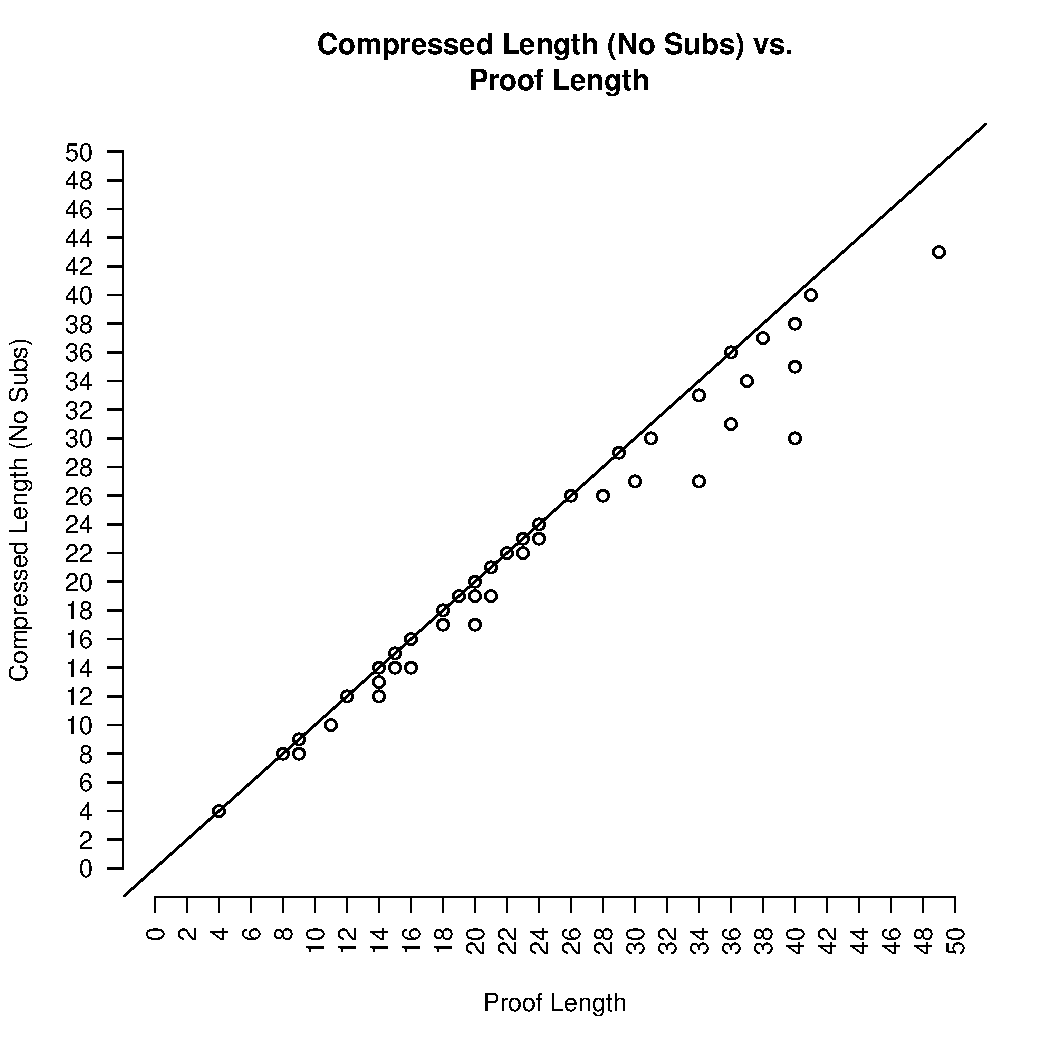
\includegraphics[scale=0.5]{images/compress_length_no_sub_vs_length.pdf}
% \end{figure}

%\begin{figure}%USED
%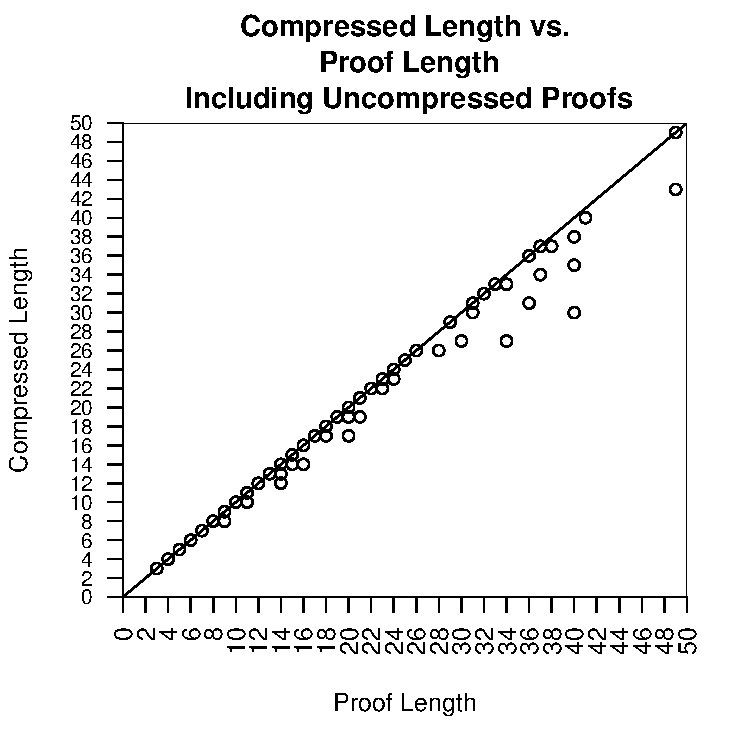
\includegraphics[scale=0.5]{images/compress_length_no_sub_vs_length_all_proofs.pdf}
%\end{figure}